\documentclass[aspectratio=169]{beamer}


% Packages
\usepackage[utf8]{inputenc}
\usepackage[T1]{fontenc}
\usepackage{lmodern}
\usepackage{amsmath, amssymb, amsfonts}
\usepackage{graphicx}
\usepackage{multimedia}
\usepackage{booktabs}
\usepackage{tikz}
\usepackage{hyperref}
\usepackage{xcolor}

% Theme
\usetheme{Madrid}
\usecolortheme{beaver} % A nice red/grey theme, looks professional
\setbeamercolor{structure}{fg=darkgray}

% Custom Commands
\newcommand{\R}{\mathbb{R}}
\newcommand{\E}{\mathbb{E}}
\newcommand{\N}{\mathcal{N}}
\newcommand{\loss}{\mathcal{L}}

% Title Info
\title[Flow Matching]{Flow Matching for 2D Data Generation}
\subtitle{From Intuition to Implementation}
\author{Arthur Courselle, Baptiste Villeneuve, Eugénie Beauvillain \texorpdfstring{\\}{, } Flavien Geoffray, Lucas Duport, Lucas Juanico}
\institute[EPITA]{SCIA 2026}
\date{\today}


\begin{document}

% Title Slide
\begin{frame}
    \titlepage
\end{frame}

% Table of Contents
\begin{frame}{Outline}
    \tableofcontents
\end{frame}

% ========================================
% Section 1: Introduction & Baseline
% Orateur: Eugenie
% ========================================
\section{Introduction \& Baseline}

% ========================================
% Section 2: Flows Continus
% Orateur: Lucas Duport
% ========================================
\section{Flows Normalisants Continus}
\begin{frame}{Flow Discret vs Flow Continu}
    \centering
    \includegraphics[width=0.9\textwidth]{imgs/discrete-vs-continuous.png}
    

\end{frame}

\begin{frame}{The Probability Flow ODE}
    \centering
    \begin{block}{Ordinary Differential Equation (ODE)}
        \centering
        \Large
        \[
        \frac{d}{dt} \phi_t(x) = v_t(\phi_t(x))
        \]
    \end{block}
    \vspace{0.5cm}
    \begin{itemize}
        \item $\phi_t(x)$: The probability path (flow) from noise to data.
        \item $v_t(\cdot)$: The velocity field defined at every point $(x,t)$.
    \end{itemize}
\end{frame}

\begin{frame}{Flow Matching Intuition}
    \begin{columns}
        \column{0.5\textwidth}
        \begin{itemize}
            \item Learning a \textbf{conditional velocity field} $v_t(x)$.
            \vspace{0.3cm}
            \item \textbf{Objective:} Push noise towards the data structure.
            \vspace{0.3cm}
            \item \textbf{Architectural Freedom:} The network $v_\theta$ no longer needs to be invertible! 
            \vspace{0.1cm}
            \begin{itemize}
                \item[$\rightarrow$] We can use a simple MLP or a U-Net for example.
            \end{itemize}
        \end{itemize}

        \column{0.5\textwidth}
        \centering
        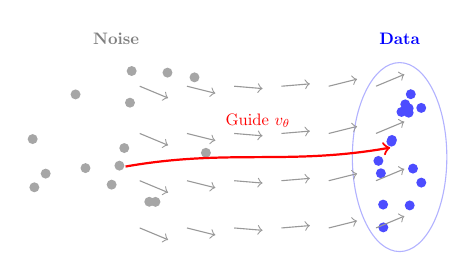
\begin{tikzpicture}[scale=0.6, transform shape]
            % Bruit (Gris) à gauche
            \node[font=\bfseries, gray] at (0, 4.5) {Noise};
            \foreach \i in {1,...,15} {
                \fill[gray!70] ({2*rand}, {2*rand + 2}) circle (3pt);
            }
            
            % Données (Bleu) à droite
            \node[font=\bfseries, blue] at (6, 4.5) {Data};
            \foreach \i in {1,...,15} {
                \fill[blue!70] ({6 + 0.5*rand}, {2 + 1.5*rand}) circle (3pt);
            }
            \draw[blue!30, thin] (6, 2) ellipse (1cm and 2cm); % Forme vague des données
            
            % Champ de vecteurs (Flèches)
            \foreach \x in {0.5, 1.5, ..., 5.5} {
                \foreach \y in {0.5, 1.5, ..., 3.5} {
                   \draw[->, black!40, thin] (\x, \y) -- ++(0.6, {0.1*(\x-3)});
                }
            }
            
            % Une trajectoire exemple
            \draw[->, red, thick] (0.2, 1.8) to[out=10, in=190] (5.8, 2.2);
            \node[red, above] at (3, 2.5) {Guide $v_\theta$};
            
        \end{tikzpicture}
    \end{columns}
\end{frame}


% ========================================
% Section 3: Théorie du Flow Matching
% Orateur: Arthur
% ========================================
\section{Théorie du Flow Matching}
\begin{frame}{Flow Matching}
Let $x_1 \sim q(x_1)$ from which we only have access to data samples.\\

Let $p_t$ be a probability path such that $p_0=p$ is a the standard normal distribution $p(x) = \mathcal{N}(x | 0, I)$, and $p_1(x) \approx q(x)$.

\begin{block}{Flow Matching (FM) objective}
\begin{equation}
    \mathcal{L}_{\text{FM}}(\theta) = \mathbb{E}_{t \sim \mathcal{U}[0,1],x\sim p_t(x)}\| v_t(x)-u_t(x) \|^2
\end{equation}
$\theta$ : the learnable parameters of $v_t$.
\end{block}
\end{frame}

\begin{frame}{Conditional Flow Matching}
Let $p_t(x|x_1)$ such that $p_0(x|x_1) = p(x)$ and $p_1(x|x_1) = \mathcal{N}(x | x_1, \sigma^2I)$. \\
\hspace{1cm}

The marginal probability $p_t(x)$ is given by \boxed{$p_t(x) = \int p_t(x|x_1) q(x_1) dx_1$}. \\
\hspace{1cm}

To find $u_t(x)$, we derive $p_t(x)$ with respect to $t$ and apply the continuity equation ($\frac{\partial p_t(x)}{\partial t} + \nabla \cdot \left[ u_t(x) p_t(x) \right] = 0$):
\begin{align}
\frac{\partial p_t(x)}{\partial t} &= \int \frac{\partial p_t(x|x_1)}{\partial t} q(x_1) \, dx_1 \\
&= -\nabla \cdot \left[ \int u_t(x|x_1) p_t(x|x_1) q(x_1) \, dx_1 \right] \\
u_t(x) p_t(x) &= \int u_t(x|x_1) p_t(x|x_1) q(x_1) \, dx_1 \\
u_t(x) &= \int u_t(x|x_1) \frac{p_t(x|x_1) q(x_1)}{p_t(x)} \, dx_1
\end{align}
\end{frame}

\begin{frame}{Conditional Flow Matching}
\begin{align}
    \mathcal{L}_{\text{FM}}(\theta) &= \mathbb{E}_{t \sim \mathcal{U}[0,1],x\sim p_t(x)}\| v_t(x)-u_t(x) \|^2 \\
    &= \mathbb{E}_{t \sim \mathcal{U}[0,1],x\sim p_t(x)}\left[ \|v_t(x)\|^2 - 2.v_t(x).u_t(x) + \|u_t(x)\|^2 \right] \\
\end{align}

We focus on the term $\mathbb{E}_{t \sim \mathcal{U}[0,1],x\sim p_t(x)}\left[ \|2.v_t(x).u_t(x) \right]$ : \\
\begin{align}
    \mathbb{E}_{t \sim \mathcal{U}[0,1],x\sim p_t(x)}\left[ \|2.v_t(x).u_t(x) \right] &= 2 \int{v_t(x).u_t(x).p_t(x)dx} \\
    &= 2 \int{v_t(x). \frac{\int u_t(x|x_1) p_t(x|x_1) q(x_1)dx_1}{p_t(x)} .p_t(x)dx} \\
    &= 2 \int{\int v_t(x).u_t(x|x_1) p_t(x|x_1) q(x_1)dx_1dx} \\
    &= 2 . \mathbb{E}_{x \sim p_t(x|x_1), x_1 \sim q(x_1)}\left[ \ v_t(x).u_t(x|x_1) \right] \\
\end{align}
\end{frame}

\begin{frame}{Conditional Flow Matching}
\small
\begin{align}
    \mathcal{L}_{\text{FM}}(\theta) &= \mathbb{E}_{t \sim \mathcal{U}[0,1],x\sim p_t(x)}\left[ \|v_t(x)\|^2 - 2.v_t(x).u_t(x) + \|u_t(x)\|^2 \right] \\
    &= \mathbb{E}_{x\sim p_t(x|x_1), x_1 \sim q(x_1)}\left[ \|v_t(x)\|^2 - 2.v_t(x).u_t(x|x_1) + \|u_t(x|x_1)\|^2 + \|u_t(x)\|^2  - \|u_t(x|x_1)\|^2 \right] \\
    &= \mathbb{E}_{x\sim p_t(x|x_1), x_1 \sim q(x_1)}\left[ \|v_t(x) - u_t(x|x_1)\|^2 + \|u_t(x)\|^2  - \|u_t(x|x_1)\|^2 \right] \\
\end{align}

Since $u_t(\dot)$ does not have any impact on the weights, we can rewrite the FM objective as :
\begin{block}{Conditional Flow Matching (CFM) objective}
\begin{align}
    \mathcal{L}_{\text{CFM}}(\theta) &= \mathbb{E}_{x\sim p_t(x|x_1), x_1 \sim q(x_1)}\left[ \|v_t(x) - u_t(x|x_1)\|^2 \right]
\end{align}
\end{block}
\end{frame}


\begin{frame}{Optimal Transport}
We consider the flow : $\psi_t(x_0) = \sigma_t(x_1)x_0 + \mu_t(x_1)$ with $u_t(x_1) = tx_1$ and $\sigma_t(x_1) = 1 - t$.

\hspace{1cm}

We differentiate : 
\begin{align}
    \frac{\partial}{\partial t} \psi_t(x_0) &= \frac{\partial}{\partial t} ((1-t)x_0 + tx_1) \\
    &= \frac{\partial}{\partial t} (x_0 - tx_0 + tx_1)\\
    &= \boxed{x_1 - x_0}\\
\end{align}
\end{frame}

\begin{frame}{Optimal Transport}

We recall : $\frac{\partial}{\partial t} \psi_t(x_0) = u(\psi_t(x_0) | x_1)$ \\

\hspace{1cm}

We can now rewrite the objective as :

\begin{block}{Optimal Transport objective}
\begin{align}
    \mathcal{L}_{\text{OT}}(\theta) &= \mathbb{E}_{x_0\sim p_0(x_0), x_1 \sim q(x_1)}\left[ \|v_t(\psi_t(x_0)) - (x_1 - x_0) \|^2 \right]
\end{align}
\end{block}

We then just need to train a neural network $v_\theta(x, t)$ to approximate the target vector field.
\end{frame}


% ========================================
% Section 4: Implémentation - Optimal Transport
% Orateur: Flavien
% ========================================
\section{Implémentation: Optimal Transport \& Sampling}

\begin{frame}{Defining the Probability Path}
    \begin{columns}
        \column{0.6\textwidth}
        \textbf{The Goal:} 
        We need to define a path for a particle to move from Noise ($x_0$) to Data ($x_1$).
        
        \vspace{0.5cm}
        
        \textbf{Optimal Transport}
        We choose the simplest geometric path: the \textbf{straight line}.
        
        \begin{block}{Interpolation Formula}
            $$ x_t = (1 - t)x_0 + t x_1 $$
        \end{block}
        
        \column{0.4\textwidth}
        \centering
        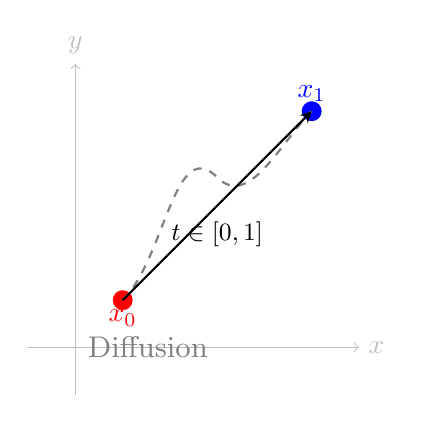
\begin{tikzpicture}[scale=1.2]
            % Axes
            \draw[->, lightgray] (-0.5,0) -- (3,0) node[right] {$x$};
            \draw[->, lightgray] (0,-0.5) -- (0,3) node[above] {$y$};
            
            % Points
            \fill[red] (0.5, 0.5) circle (3pt) node[below] {$x_0$};
            \fill[blue] (2.5, 2.5) circle (3pt) node[above] {$x_1$};
            
            % Diffusion models (dashed curve)
            \draw[dashed, gray, thick] (0.5, 0.5) to[out=45, in=135] (1.5, 1.8) to[out=315, in=225] (2.5, 2.5) node[midway, right] {\small Diffusion};
            
            % Flow matching (solid line)
            \draw[thick, ->, >=stealth] (0.5, 0.5) -- (2.5, 2.5) node[midway, above left] {};
            
            % Time label
            \node at (1.5, 1.2) {\small $t \in [0, 1]$};
        \end{tikzpicture}
        \end{columns}
\end{frame}

\begin{frame}{The Regression Target}
    The neural network needs to learn the \textbf{velocity field} $v_\theta(x, t)$ that generates this path.
    
    \vspace{0.5cm}
    
    Since the path is a straight line, the velocity is the time derivative:
    
    $$ u_t(x|x_1) = \frac{d}{dt} x_t = \frac{d}{dt} \left( (1 - t)x_0 + t x_1 \right) $$
    
    \vspace{0.5cm}
    
    \begin{alertblock}{The Key Advantage}
        The target velocity is \textbf{constant}:
        $$ u_t = x_1 - x_0 $$
    \end{alertblock}
    
    \vspace{0.3cm}
    $\Rightarrow$ The network learns a stable, constant direction for each pair, which is easier than learning a curved diffusion path.
\end{frame}

\begin{frame}{Sampling with Euler Method}
    \textbf{Inference:} Starting from noise $x_0$, we follow the learned velocity field.
    
    \begin{columns}
        \column{0.55\textwidth}

        We use the \textbf{Euler Integration}:
        $$ x_{t+dt} = x_t + v_\theta(x_t, t) \cdot dt $$
        
        \vspace{0.2cm}
        
        \textbf{Why it works well?}
        \begin{itemize}
            \item The learned trajectories are nearly straight (Optimal Transport).
            \item Low discretization error.
            \item Fast generation ($N=10$ to $20$ steps).
        \end{itemize}

        \column{0.4\textwidth}
        \begin{algorithm}
            \footnotesize
            \textbf{Algorithm: Sampling}
            \begin{enumerate}
                \item $x \leftarrow \text{SampleNoise}()$
                \item $dt \leftarrow 1/N$
                \item \textbf{For} $i = 0$ to $N-1$:
                \begin{itemize}
                    \item $v \leftarrow \text{Model}(x, t)$
                    \item $x \leftarrow x + v \cdot dt$
                    \item $t \leftarrow t + dt$
                \end{itemize}
                \item \textbf{Return} $x$
            \end{enumerate}
        \end{algorithm}
    \end{columns}
\end{frame}


% ========================================
% Section 5: Implémentation - Code
% Orateur: Lucas Juanico
% ========================================
\section{Implémentation: Code \& Architecture}
\begin{frame}{Flow Matching Training Loop}
    \small
    \textbf{Algorithm}
    \begin{enumerate}
        \item Sample a minibatch $x_1 \sim p_{\text{data}}$
        \item Sample noise $x_0 \sim \mathcal{N}(0,I)$ and time $t \sim \mathcal{U}[0,1]$
        \item Interpolate:
        \[
            x_t = (1 - t)x_0 + t x_1
        \]
        \item Compute target vector field:
        \[
            u_t = x_1 - x_0
        \]
        \item Predict vector field  $\hat{u}_t = v_\theta(x_t,t)$
        \item Calculate $MSE(\hat{u}_t, u_t)$
        \item Backpropagate and optimize model
    \end{enumerate}
\end{frame}
    
\begin{frame}{Qualitative Results: CIFAR-10}
    \begin{center}
        \includegraphics[width=0.7\textwidth]{imgs/reconstruction_CIFAR10_1.png}
    \end{center}
    \begin{itemize}
        \item Scaling to high-dimensional data using a \textbf{U-Net} backbone.
        \item The model generates sharp samples by following the learned velocity field.
    \end{itemize}
\end{frame}

\begin{frame}{Qualitative Results}
    \begin{center}
        \includegraphics[width=0.7\textwidth]{imgs/reconstruction_CIFAR10_.png}
    \end{center}
\end{frame}

\begin{frame}{Qualitative Results}
    \begin{center}
        \includegraphics[width=0.7\textwidth]{imgs/reconstruction_MNIST_.png}
    \end{center}
\end{frame}


% ========================================
% Section 6: Résultats & Comparaison
% Orateur: Baptiste
% ========================================
\section{Résultats \& Comparaison}
\section{Expérimentations \& Comparaisons}

\begin{frame}{Comparaison}
    \begin{columns}
        \column{0.5\textwidth}
        \textbf{RealNVP (Baseline)}
        \begin{itemize}
            \item \textbf{Inférence :} Très Rapide ($O(K)$ couches)
            \item \textbf{Entraînement :} Plus complexe
            \begin{itemize}
                \item NLL
                \item Inversibilité
            \end{itemize}
        \end{itemize}

        \column{0.5\textwidth}
        \textbf{Flow Matching (Notre Approche)}
        \begin{itemize}
            \item \textbf{Inférence :} Plus Lente (ODE Solver)
            \item \textbf{Entraînement :} Simple \& Stable
            \begin{itemize}
                \item Convergence plus rapide
            \end{itemize}
        \end{itemize}
    \end{columns}
\end{frame}

\begin{frame}{Synthèse des Performances}
    \begin{table}[]
        \centering
        \begin{tabular}{@{}lcc@{}}
        \toprule
        \textbf{Critère} & \textbf{RealNVP} & \textbf{Flow Matching} \\ \midrule
        Vitesse d'Inférence & \textcolor{green}{\textbf{Instantanée}} & \textcolor{red}{Lente} \\
        Complexité Entraînement & \textcolor{red}{Élevée} & \textcolor{green}{\textbf{Faible (Régression)}} \\
        Stabilité Convergence & Moins stable & \textcolor{green}{\textbf{Très stable}} \\ \bottomrule
        \end{tabular}
        \caption{Tableau récapitulatif des avantages et inconvénients.}
    \end{table}
\end{frame}


% ========================================
% Conclusion
% ========================================
\begin{frame}
    \centering
    \Huge Thank You!
    \vspace{1cm}
    
    \normalsize
    \textit{Code available at: https://github.com/ArthurCourselle/FlowMatching}
\end{frame}

\end{document}
